\documentclass{report}
\usepackage{graphicx}
\usepackage[numbers]{natbib}
\begin{document}
\title{GUI for mail-merge using Erlang and Erlguten}
\author{Yuan Zhiqian}
\date{April 2011}
\maketitle
\begin{abstract}
  Klarna AB is a financial company which provides payment solutions for the e-commerce sector, and they need to generate a lot of invoices everyday, which involves a large amount of tedious work, so they need a tool to facilitate this task. The new method of invoice generating consists of two sub-process, i.e. designing templates and make mail-merging between templates and userdata。

  This project aims for implementing a system to solve the issues described above, it mainly targets on the mail-merging of templates and userdata, besides it also provides a prototype of GUI for designing the templates. The final goal is to realize the automation of invoice generating to the greatest extent, later in this report I will illustrate how far this goal is reached.

  This system involves many technique areas, the techniques mainly used are Erlang, Erlguten, Cappuccino framework, javascript, rubyonrails etc.
\end{abstract}

\tableofcontents

\chapter{Introduction}
  This chapter introducts the project by generally describing it and giving its background. At the end of this chapter, the report structure is shown.
\section{Project Overview}
  Invoice generating is always a big task for companies, finacial companies especially. The problem is not only the huge amount of the generation, but also the series of problems aroused during the procession of this repeative and tedious task. Typoes may occur, and a lot of time are wasted on the repeative inputting of data for every individual invoices. So it is always good to make this kind of task automated. However, automation has its own disadvantage, that is, the lack of human-maintaining leads to the potential flaws in typesetting, layout designing etc. So the programmer has to consider the issues which were formerly faced by marketing people who design invoices by hands. 

  Fortunately there's a tool called erlguten which we can use to help achieve the goals in typesetting, so that tasks like space management, auto-linebreaks of paragraphs are no more big issues. The question becomes how to design the system so that it can make good use of erlguten's functionality, together with its own mail-merging fucntionality, as well as to achieve the full automation from the template designing to PDF generating.

  This project is developed using many languages. The backend batch program is implemented in Erlang/OTP, and the GUI is implemented using Cappuccino framework, which is written in Objective-J, a super-set of Javascript. And the whole system is packed and connected using RubyonRails, which can be used to implement web services easily. 

  The project is maintained using git, the repository is homed on github. You can find the project and download the codes in this link: 

  https://github.com/yuanzhiqian/mailmerging\_using\_erlang\_and\_erlguten

  This report is edited using Latex typesetting software.

  During the development of this project, engineer and managers in Klarna AB has been helping me a lot with various issues. I would like to express my great appreciation to Erik Stenman who has been guiding me and prompting valuable advices, and Samir Fors who has recommended me the brilliant javascript-based web application framework -- the Cappuccino framework, and many other developers for their help. 

\section{Background}
  In this background section, two aspects will be described: the thesis background, and the technical background.
\subsection{Thesis Background}
  This thesis is initiated and sponsored by Klarna AB.

  Klarna AB is a fanancial company which provides payment solutions for the e-commerce sector, during the daily transaction, invoice generating appears to be a heavy task so it is good to make this process automated. The company is using "Klarna Online", an in-house developed system written in Erlang, to generate transaction documents. The origianl system let the marketing people manually write Erlang codes to design the layout of invoices, with the help of erlguten, which is very incovenient and what is worse is that the end users have to know a lot of technical details to be qualified for this work. Besides, according to their plan, in the invoices, transpromos need to be added as well, so now they want an improved system to replace the old one, so as to alleviate the burden of invoice generating and realize the transpromo functionality. The following goals are supposed to be achieved by the new system:

\begin{enumerate}
\item The marketing and product development departments should be able to do most of the maintenance of the document templates. (i.e. The invoice generating task is divided into two parts -- templates maintenance, and the batch of mail-merging and pdf generating, the latter is supposed to be fully automated and the former is supposed to be facilitated by providing intuitive GUI for template designing and maintaining. )
\item The system should support functionality for Transpromo and making more attractive transaction documents.
\end{enumerate}

\subsection{Technical Background}
\subsubsection{Erlguten}
  Erlguten is a system for hiqh quality typesetting, ErlGuten is free soft-ware. ErlGuten aims to produce typographic quality PDF directly from XML or from a program.\cite{erlguten03}
 
  Here is a short citation from the official introduction:

\begin{quote}
  ErlGuten is designed for the production of large and complex documents
with complex layout requirements, like newspapers or books. In ErlGuten
layout, content, and document management are considered separate issues.
Layout is template based - Content is assumed to be stored as a large num-
ber of documents in a file system or data base, document management is con-
sidered as a mapping operation which takes documents in the content data
base and maps them onto templates to produce hight quality output.\cite{erlguten03} 
\end{quote}

  Erlguten provides a bundle of methods in "pdf" module (In the new version of erlguten, the module is renamed as eg\_pdf, and some functionalities from other modules are combined into this module.), using which, the programmer can specify the layout of a pdf document and it then will be generated into pdf file by invoking the export method that erlguten provides. Erlguten also provides text and image management, which have greatly simplified the process of typesetting. 

  Besides of those described above, erlguten also defines its own typesetting formats and syntax, the user can specify layouts separately in a xml file, on the other hand, the contents are written in another xml file, with the "layout to be used" indicated, then the erlguten will do the batch for those files and generate the final pdf. The aim of this is to separate layout of a document from the contents.

  At the beginning, I adopted this functionality because during the batch process, erlguten will do the text management automatically; but later, because of the new requirements, this method has to be discarded, and I decided to directly use pdf module for pdf generating. However, the old library for the original version of my project is retained for potential uses, although the methods, which rely on that library, are deprecated. 

\subsubsection{Cappuccino Framework and Objective-J}
  Cappuccino Framework\cite{capp} is an open source framework for developing web applications that look and feel like Mac OS desktop applications. Cappuccino provides handy APIs which programmer can use to directly develop web applications without needing to concern themselves with HTML, CSS or even DOM. 

  Cappuccino is implemented using a new programming language called Objective-j, which is analogous to Objective-C in some way, like message calls etc, but it is built on Javascript and its compiler is totally written in Javascript, so programs written in Objective-j don't need any server side compilation. Objective-j inherits some design patterns from Cocoa, like delegation etc.

  Cappuccino framework provides Cocoa-like API, so that Mac OS X programmer can easily get hand on this framework.  

\section{Report structure}
  The following parts of this report will be arranged as follows:

  First the issues faced and the goals to achieve will be specified, then in the Implementation chapter, the system's structure is shown and each component is described. The Evaluation chapter will show the result of tests on the system to see how well the problems are solved. And I will state the future works to be done on improving the mail-merging component and extending the GUI prototype. Finally I'll make a summary on the project.

\chapter{Problem Description}
  This chapter first describes the issues faced, then it will describe the goals and motivation. At the end, I will specify the method I use.

\section{Issues}
  The automation of invoice generating involves many aspects, so there're a lot of thing I need to do research on. 

  First, the company uses mail-merging to achieve automation, that means it's hard to use erlguten's original pdf-generating method, because they follow different logics. Second, I need to define the format of templates by myself, and I also need to consider the conversion from GUI elements to xml-based template files. The third, as the company requires, a GUI is preferred, but because of the limitation of time, it is hardly possible to build such a sophisticated GUI from scratch. So what I need to do is to try to find a framework to facilitate the work. 

  Besides of these, I also need to think about how to combine every components and make the whole system run on good condition -- if everything works perfect, the end user should see nothing more than the GUI itself, so they may not expect something like a exclamation saying that "an error occurred, templates are not in the right directory", those confusing internal errors do exist when trying to make every individual components cooperate with each other.

  Moreover, how to make the GUI intuitive and convenient to use is also a big issue, although it is not mandatory to provide a fully-functioning GUI, but it is always good to at least bring up some good ideas in the prototype. 

  And there are some requirements on the functionalities to implement as well, which will be described in the next section.

\section{Goals and motivation}

  Because the requirement of automation, the system adopts mail-merging technique. Along with the requirements from Klarna company, the goals are as follows,

\begin{itemize}
\item Implement the mail-merging functionality which can replace dynamic fields in the templates with specified user data.
\item The system should be able to deal with text, image, table and list items.
\item The system should be able to estimate the length of document, and select the right template among the alternatives.
\end{itemize}

\section{Method Used}
  Mail-merge technique is adopted to make the system dynamically process large amount of user data. To mark up a dynamic field, I introduce escape characters. I use "\#" to indicate a dynamic field. During a mail-merging process, the system checks the template file, extracts dynamic fields(also called as "parameter") from the template, and make a query in the user data files. The system then substitute the field with the actual data it finds, or send out an error message in case the parameter's name can't be found in user data files. 

  The mail-merge of text and image are performed in the same way, i.e. replace the parameter with the actual data found in the user data files. As for image, the data would be the path where images are stored.

  As for tables and lists, things are different. There are two reasons, first of all, table and list need to follow special format and layout; second, a table item is dynamically expanding, you never know how many rows are needed until you access the user data files. However, the aim of automation is to let the user not have to know about the actual user data, because only the program needs to access the user data. So in the template, a table is simply indicated as a table item, with some information of formats and a index referring to the table data in the user data files to present. So the mail-merge of a table item is done in this way: the system find out the table items, and check its name, then the system look up this name in the user data files. When they system finds the right data, it concatenates the data with the format information in the template file, this merged segment will later be process by the PDF generation module, in that phase, indicated columns will be chosen to print and format information, if any, will be parsed and performed on the printing procedure.

  The list is easier to process, because no dynamic-length lists are required, we just need to define the items of lists in the template file, and replace those items in the same way as dynamic texts.

  The GUI is implemented based on cappuccino framework, it is a outstanding tool to design web applications. The GUI is built from a tutorial provided by the website "http://www.nice-panorama.com/Programmation/cappuccino/", so it inherits a lot of the original layouts of the tutorial. The GUI allow users to create as many templates as they want(but due to some restrictions, the amount of templates may be limited below three. This will be explained in the next chapter), the users edit the template as if they are using painting board, now the GUI allows the users to draw frames to indicate the boundaries of items, if time allows, I may add the functions of editing view so that the user can type in contents and attributes in the frame, in the future's work, some auxiliary tools like rulers and coordination tags may be provided to aid the alignments. When the users finish editing, they can generate xml files for the templates by pressing the corresponding button, when everything is ready, the user can press the generate pdf button to export pdf files. This function is done by making a call to the back-end modules, i.e. the parts described above.

\chapter{Implementation}
  This chapter describes the technical solution of this system. 
\section{System Environment}
\begin{itemize}
\item Ubuntu Linux 10.10
\item Erlang R14B02 (erts-5.8.3)
\item Erlguten 
\item Cappuccino framework 0.9
\item Javascript
\item RubyonRails 3.0.7
\end{itemize}
\section{System Structure}
  Figure \ref{fig1} illustrates the system structure in graphics. As described in figure \ref{fig1}, the user data are first retrieved from database and automatically converted into XML files, but this process is done outside of the system. Then the marketing people design templates according to the requirements using the GUI running in the web browser. By pressing the "save templates" button, the templates will be sent to the server by making an XMLHttpRequest, which will be processed by the web service written in rubyonrails. When this is done, the user would like to generate pdfs, and he will press "generate pdf" button to send another XMLHttpRequest, when the server receive the request, it will execute the script to call the mail-merge functions and do the mail-merge, generating invoices as pdf files. 

\begin{figure}[p]
\centering
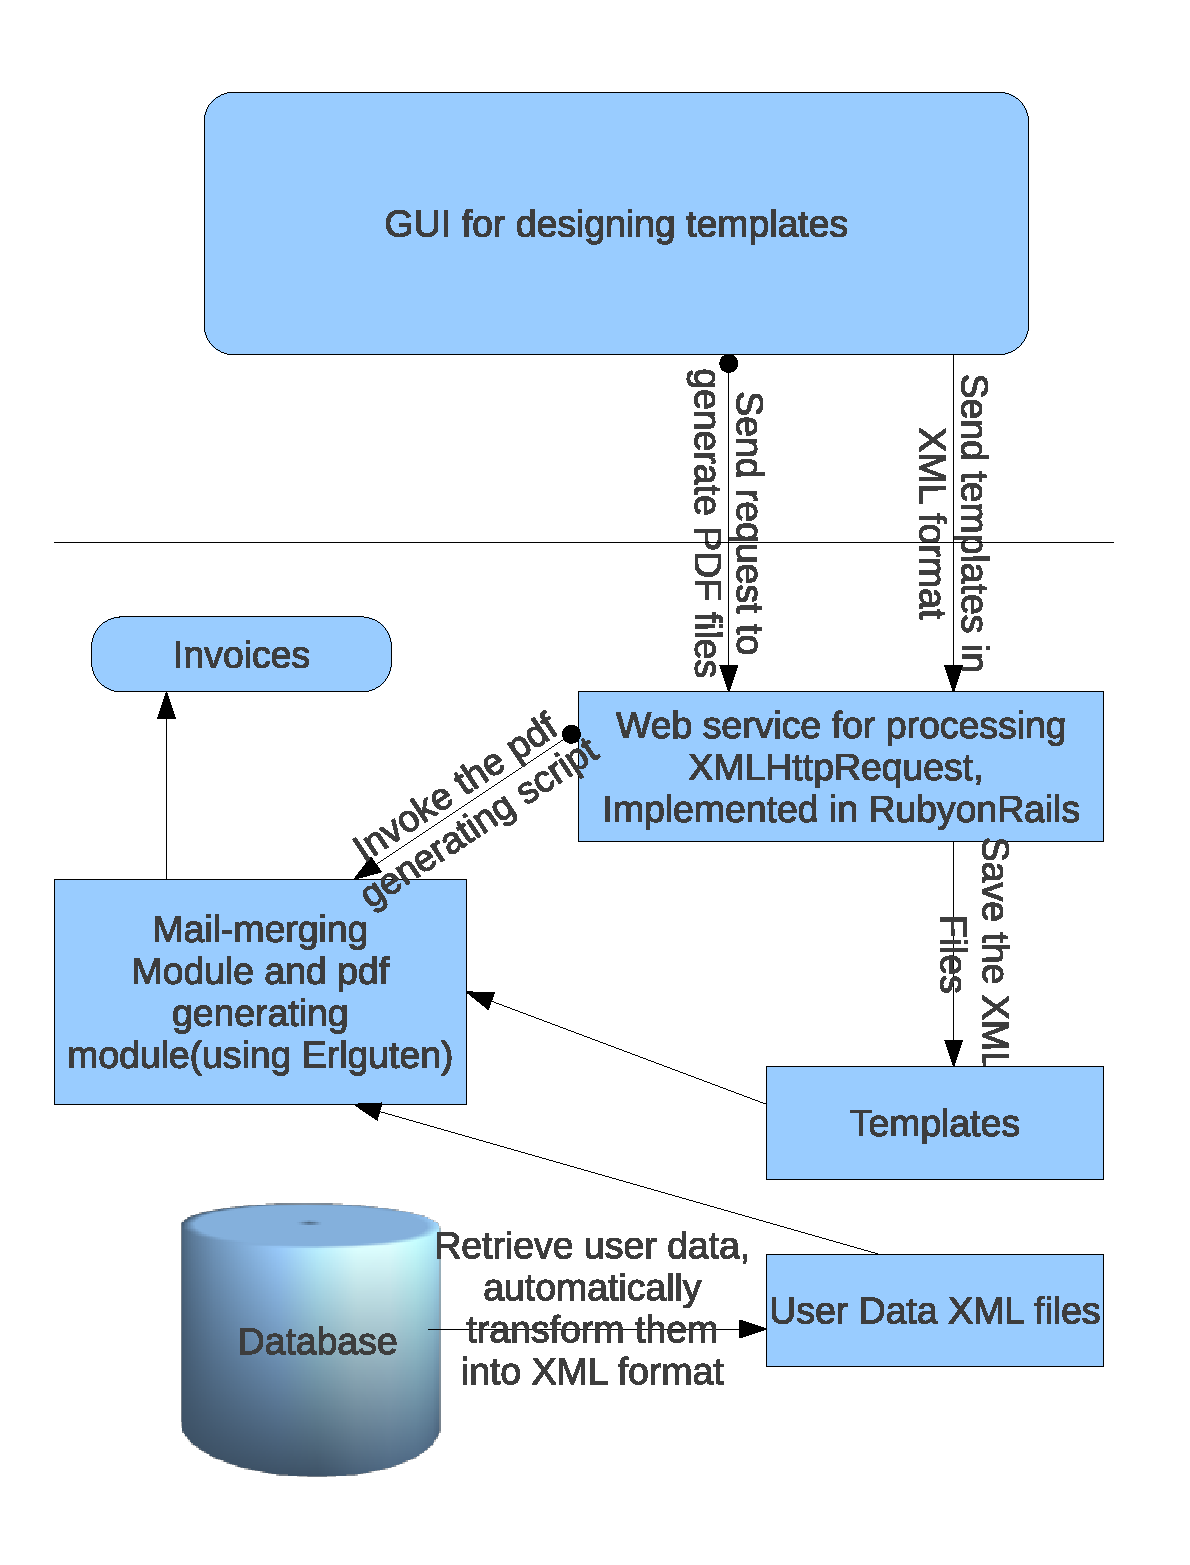
\includegraphics[scale=0.5]{systemstructure.eps}
\caption{System Structure illustrated in graphic form}
\label{fig1}
\end{figure}

\section{Implementation for each part}
\subsection{Template Format}
  I would like to use a sample to explain the format of template:

\begin{quote}

$<$?xml version="1.0" ?$>$
$<$template count = "3" alt2 = "N/A" alt3 = "N/A"$>$
$<$paper name = "first" class = "front"$>$

  $<$frame name = "trademark" class = "img" x = "48" y = "30" width = "94" height = "20" grid = "true" bg = "default" font = "N/A" fontsize = "N/A" paraIndent = "N/A" maxlines = "N/A" continue = "N/A" break = "N/A"$>$\#tm$<$/frame$>$

  $<$frame name = "hello" class = "text" x = "48" y = "140" width = "177" height = "127" grid = "true" bg = "1.0,0.0,0.0" font = "Times-Roman" fontsize = "15/20" paraIndent = "0" maxlines = "4" continue = "none" break = "true"$>$Hello \#name, here is your invoice, this is a new version of template.$<$/frame$>$

  $<$frame name = "shoppinglist" class = "list" x = "48" y = "280" width = "177" height = "140" grid = "true" bg="default" font = "Times-Roman" fontsize = "14/20" paraIndent="0" maxlines = "30" continue="none" break="true"$>$

\{ul\}\{li\}\#first\{/li\}\{li\}\#second\{/li\}\{li\}\#third\{/li\}\{/ul\}$<$/frame$>$


  $<$frame name = "shoppingtable" class = "table" x = "48" y = "450" width = "177" height = "100" grid = "false" bg="default" font = "Times-Roman" fontsize = "12/24" paraIndent="0" maxlines = "30" continue="shoppingtable2" break="true"$>$

\{table columns = \{goods, count, price, place\}\}

\{tr\}\{th\}\#goods\{/th\}\{th\}count\_col?\{/th\}

\{th\}\$price?\{/th\}\{th\}place\{/th\}\{/tr\}\{/table\}$<$/frame$>$

$<$/paper$>$

$<$paper name = "second" class = "middle"$>$
  
  $<$frame name = "trademark" class = "img" x = "48" y = "30" width = "94" height = "20" grid = "true" bg = "default" font = "N/A" fontsize = "N/A" paraIndent = "N/A" maxlines = "N/A" continue = "N/A" break = "N/A"$>$\#tm$<$/frame$>$

  $<$frame name = "shoppingtable2" class = "table" x = "48" y = "140" width = "177" height = "640" grid = "false" bg="default" font = "Times-Roman" fontsize = "12/24" paraIndent="0" maxlines = "30" continue="shoppingtable3" break="true"$>$

@shoppingtable$<$/frame$>$

  $<$frame name = "faq" class = "text" x = "300" y = "128" width = "280" height = "153" grid = "true" bg = "default" font = "Times-Roman" fontsize = "12/24" paraIndent = "0" maxlines = "6" continue = "none" break = "true"$>$Question and Answer: \#text$<$/frame$>$

$<$/paper$>$

$<$paper name = "third" class = "end"$>$
  
  $<$frame name = "trademark" class = "img" x = "48" y = "30" width = "94" height = "20" grid = "true" bg = "default" font = "N/A" fontsize = "N/A" paraIndent = "N/A" maxlines = "N/A" continue = "N/A" break = "N/A"$>$\#tm$<$/frame$>$

  $<$frame name = "shoppingtable3" class = "table" x = "48" y = "140" width = "177" height = "400" grid = "false" bg="default" font = "Times-Roman" fontsize = "12/24" paraIndent="0" maxlines = "30" continue="none" break="true"$>$@shoppingtable2$<$/frame$>$

  $<$frame name = "slip" class = "img" x = "0" y = "550" width = "600" height = "250" grid = "true" bg = "default" font = "N/A" fontsize = "N/A" paraIndent = "N/A" maxlines = "N/A" continue = "N/A" break = "N/A"$>$\#slip$<$/frame$>$

$<$/paper$>$

$<$/template$>$ 

\end{quote}

  As you may notice, there are three "paper" nodes under the root node "template". But this is not always the case, it would take many words to explain this: basically, an invoice consists of trademarks, text contents, tables, graphic elements and a slip to indicate the payment details, and the slip is supposed to be always placed at the end of the document. And an invoice always has a table as well, but the length or the table is not sure of when the marketing people designs the templates, so the number of pages needed is unknown too, therefore they should prepare three kinds of templates to cover all the cases that may occur -- they are: one-page template, to be used for the documents that only have one page (the slip is at the bottom of the page); two-page template, to be used for the documents that only have two pages (the slip is at the bottom of the last page); three-page template, to be sued for the documents that have more than two pages (the slip is at the bottom of the last page, and there's also a "middle page template" to define the pattern of the pages between the front page and the end page). 

  And because that the template may be one-page template, two-page template, or three-page template, there should be attributes to indicate the alternative templates if the current template doesn't fit. So the "template" node contains "alt2" and "alt3" attributes for this use.

  In each "paper" node, there are many frames. Currently there are four kinds of frames: text frame which denotes a flow of normal texts, and image, table, list frames which denotes the corresponding items. The type of frames are specified by the "class" attribute. The attributes of frame is listed as follows:

\begin{itemize}
\item name, the name of frame
\item class, the type of frame
\item x, the x coordinate of the top left corner of frame
\item y, the y coordinate of the top left corner of frame
\item width, the width of frame
\item height, the height of frame
\item grid, whether or not the grids are needed to be shown
\item bg, the background color of frame
\item font, the font of texts in the frame
\item fonsize, the size of texts in the frame
\item paraIndent, the indent of paragraphs
\item maxlines, the number of lines needed
\item continue, deprecated attribute
\item break, deprecated attribute
\end{itemize}

  The content of four kinds of frames are as follows:

  \textbf{text}: the content of a text frame node contains static texts as well as dynamic texts. The dynamic texts are denoted beginning with a \# mark. A sample of the content is like this: 

  $<$frame .... $>$ Hello \#name, the amount you need to pay is \#price $<$/frame$>$

  \textbf{image}: the content of a image frame node contains a parameter, which is to be replaced by a string which indicates the path where image files are stored, the replacement happens during mail-merge process. The parameter is just a dynamic text. This is a sample of a image frame:

  $<$frame .... $>$ \#trademark $<$/frame$>$

  \textbf{table}: the content of a table frame node is defined in a special format. Here is a sample of a table frame:

\{table columns = \{goods, count, price, place\}\}

\{tr\}\{th\}\#goods\{/th\}\{th\}count\_col?\{/th\}

\{th\}\$price?\{/th\}\{th\}place\{/th\}\{/tr\}\{/table\}

  As you may have noticed, the format of a table is very similar with that in HTML language, however I just borrow the idea from HTML and there're some differences between them. First a table has column attribute to indicate the columns selected to print out, because there may be many columns in a table in the user data files, and different template may want different columns to show, that's why we need such an attribute here. And a \{tr\}\{/tr\} couple denotes one row in the table, however, here it is only used to contain the table headers. Because some tables may have no headers, and some tables may have headers with different names, thus I decided that the user should be able to explicitly specify the headers. 

  \textbf{list}: the content of a list frame node is like this:

\{ul\}\{li\}\#first\{/li\}\{li\}\#second\{/li\}\{li\}\#third\{/li\}\{/ul\}

  The format of list definition is also borrowed from HTML language, just using different marks. The content of list is also dynamic texts, its substitution method is the same as described above. 
  
\subsection{Mail-merging and pdf generating algorithm}

  The mail-merge and pdf generating functionality is the main component in this system, figure \ref{fig2} shows the flow of this process. 

\begin{figure}[p]
\centering
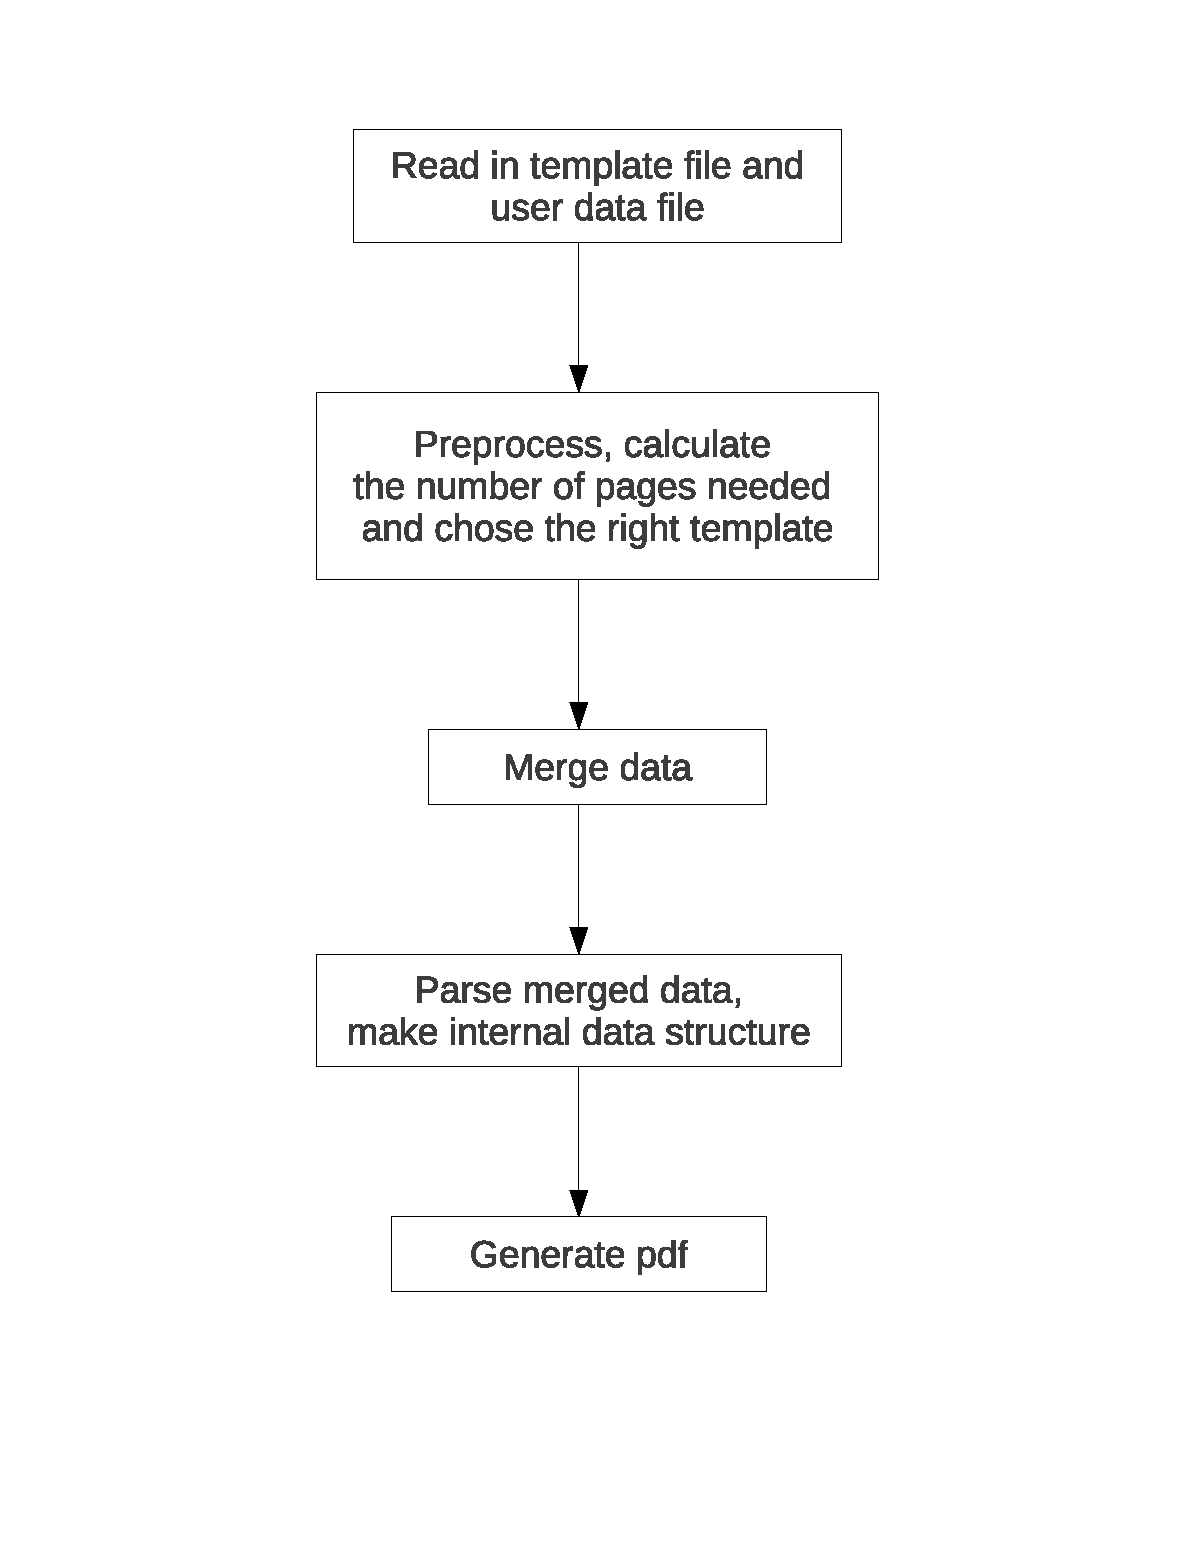
\includegraphics[scale=0.5]{mailmergeprocess.eps}
\caption{Flow chart of mail-merge process}
\label{fig2}
\end{figure}

\subsection{GUI Implementation}
\subsubsection{Template Generating}
\subsection{Combination of GUI and back-end system}

\chapter{Evaluation}
\section{Mail-merging}
\subsection{Text}
\subsection{Image}
\subsection{Table}
\subsection{List}
\section{GUI}

\chapter{Future work}
\section{Mail-merging part}
\section{GUI part}

\chapter{Summary and Conclusions}

\begin{thebibliography}{9}
\bibitem{erlguten03}Erlguten repo, 2003. Erlguten repository on google code. http://code.google.com/p/erlguten/
\bibitem{capp} Cappuccino website. http://cappuccino.org/
\end{thebibliography}

\end{document}
